\documentclass[varwidth]{standalone}
\usepackage{tikz}
\begin{document}
\begin{varwidth}{\linewidth}
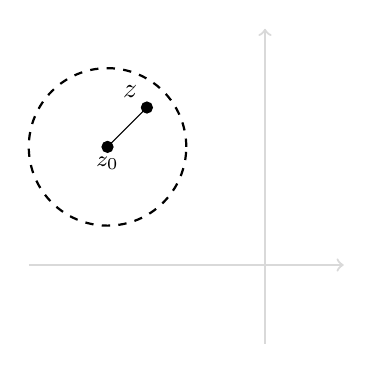
\begin{tikzpicture}
\draw[->, thick, gray!30] (-3,0) --  (1,0);% node[right]{$\mathsf{Re}$} ;
\draw[->,thick, gray!30] (0,-1) -- (0,3);% node[above]{$\mathsf{Im}$};
\draw[thick,dashed] (-2,1.5) circle(1);    
%\draw[<->,dashed] (2,2) -- %node[midway,above]{$k$}
(3.5,2);
%\draw[fill]  (2,2) circle(2pt);
\draw[fill]  (-2,1.5) circle(2pt) node[below,font=\footnotesize]{$z_0$} -- (-1.5,2) circle(2pt) node[above left] {$z$};
%\draw (2,2) -- (2.75,2.75);
%\draw (2.75,2.75) node[above left]{$z$};
%\draw[fill]  (2.75,2.75) circle(2pt);
%\draw[thick] (1.25,1.5) -- (1.5,2) -- (1.75,1.5) -- (1.25,1.5);
\end{tikzpicture}
\end{varwidth}
\hspace{2cm}
\begin{varwidth}{\linewidth}
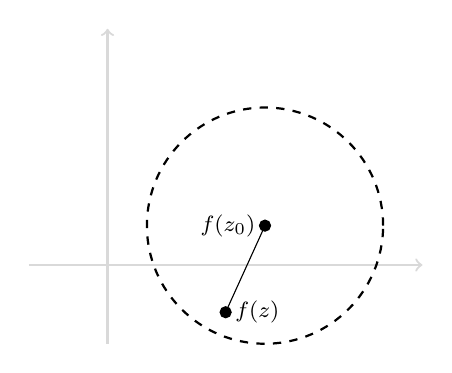
\begin{tikzpicture}
\draw[->, thick, gray!30] (-1,0) --  (4,0);% node[right];%{$\mathsf{Re}$} ;
\draw[->,thick, gray!30] (0,-1) -- (0,3);% node[above];%{$\mathsf{Im}$};
\draw[dashed,thick] (2,0.5) circle (1.5) ;
\draw[fill] (2,0.5) circle (2pt) node[left,font=\footnotesize] {$f(z_0)$} -- (1.5,-0.6) circle (2pt) node[right,font=\footnotesize] {$f(z)$};
\end{tikzpicture}
\end{varwidth}
\end{document}